\documentclass[11pt]{standalone}

\usepackage{fontspec}
\usepackage{unicode-math}

\setmainfont{TeX Gyre Pagella}
\setsansfont{Linux Biolinum O}
\setmathfont{TeX Gyre Schola Math}

\usepackage{ifthen}
\usepackage{amsmath}

\usepackage[d]{esvect}
\usepackage[svgnames]{xcolor}
\usepackage{tikz}
\usetikzlibrary{shapes.misc}
\usetikzlibrary{arrows,arrows.meta}
\usetikzlibrary{calc,intersections, patterns, math}

\definecolor{pfeil}{RGB}{168,167,167}
\definecolor{salmon}{RGB}{250,128,114}
\definecolor{petrol}{RGB}{0, 118, 136}
\definecolor{darkgoldenrod}{RGB}{184, 134, 11}
\colorlet{petrol-lighter}{petrol!40}
\colorlet{darkgoldenrod-lighter}{darkgoldenrod!40}

\tikzset{>={Stealth[scale=1.25]}}

\begin{document}

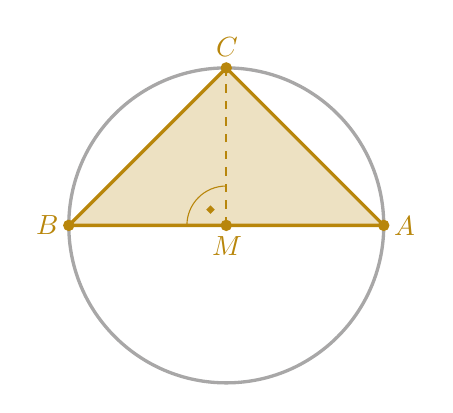
\begin{tikzpicture}[pfeil, very thick]
			
	\draw[very thick] (0,0) circle (2);

	\draw[thick, dashed, darkgoldenrod] (0,0) -- (0,2);
	\draw[thin, darkgoldenrod] (0,0.5) arc (90:180:0.5);
	\draw[darkgoldenrod, fill] (-0.2, 0.2) circle(0.025);
	\draw[draw=darkgoldenrod, fill=darkgoldenrod, fill opacity=0.25, very thick] (-2,0) -- (2,0) -- (0,2) -- cycle;

	\draw[darkgoldenrod, fill] (-2,0) circle (0.05) node[left] {$B$};
	\draw[darkgoldenrod, fill] (2,0) circle (0.05) node[right] {$A$};
	\draw[darkgoldenrod, fill] (0,2) circle (0.05) node[above] {$C$};
	\draw[darkgoldenrod, fill] (0,0) circle (0.05) node[below] {$M$};
\end{tikzpicture}			

\end{document}
